\documentclass[conference]{IEEEtran}
\IEEEoverridecommandlockouts
% The preceding line is only needed to identify funding in the first footnote. If that is unneeded, please comment it out.
\usepackage{cite}
\usepackage{amsmath,amssymb,amsfonts}
\usepackage{algorithm}
\usepackage{algorithmic}
\usepackage{graphicx}
\graphicspath{{evals/data/metrics/figures/final/}}
\usepackage{textcomp}
\usepackage{xcolor}
\usepackage{array}
\usepackage{booktabs}
\usepackage[most]{tcolorbox}

% Churkin Protocol: Color Palette (Harmonious & Minimal)
\definecolor{churkinpurple}{RGB}{94,45,121}    % #5E2D79 (for State)
\definecolor{statusgreen}{RGB}{34,139,34}      % #228B22 (Green for True - Success)
\definecolor{statusred}{RGB}{255,99,71}       % #FF6347 (Light Red/Tomato for False - Stop/Suppressed)
\def\BibTeX{{\rm B\kern-.05em{\sc i\kern-.025em b}\kern-.08em
    T\kern-.1667em\lower.7ex\hbox{E}\kern-.125emX}}

\begin{document}

\title{EXAIM: Explainable AI Middleware for Real-Time Multi-Agent Clinical Decision Support\thanks{This work was supported by Dakota State University.}}

\author{\IEEEauthorblockN{Abem Kibatu Woldesenbet}
\IEEEauthorblockA{\textit{The Beacom College of Computer \& Cyber Sciences} \\
\textit{Dakota State University}\\
Madison, SD, USA \\
abem.woldesenbet@trojans.dsu.edu}
\and
\IEEEauthorblockN{Andy Behrens, PhD}
\IEEEauthorblockA{\textit{Information Systems, College of Business \& Information Systems} \\
\textit{Dakota State University}\\
Madison, SD, USA \\
andy.behrens@dsu.edu}
}

\maketitle

\begin{abstract}
Multi-agent Large Language Models (LLMs) offer diverse diagnostic perspectives but generate verbose, interleaved reasoning traces that overwhelm clinicians. We present EXAIM, a middleware artifact that transforms streaming multi-agent reasoning into structured, schema-constrained summaries aligned with standard clinical communication protocols (SBAR (Situation, Background, Assessment, Recommendation) / SOAP (Subjective, Objective, Assessment, Plan)). In contrast to heuristic turn-based approaches, EXAIM employs semantic event-driven buffering to trigger summary updates when the stream indicates clinically meaningful semantic transitions (e.g., relevant, novel, completed reasoning units; topic shifts; critical alerts), thereby decoupling update frequency from generation rate.

In a controlled ablation study on rare-disease diagnostic traces, EXAIM reduces update frequency by 75\% compared to non-filtering baselines (11.65 vs. 46.4 updates per case) while maintaining high information density under strict, clinically aligned length constraints. The system achieves strict schema compliance (96.8\%) and a median latency of 1.22~s, validating its computational feasibility for real-time deployment. These results demonstrate that event-driven, schema-constrained summarization can effectively mediate the tension between information volume and interruption frequency, offering a tunable architectural control for clinical information flow.
\end{abstract}

\begin{IEEEkeywords}
Clinical decision support, Event-driven summarization, Explainable AI, Multi-agent systems, Real-time summarization, Schema-constrained summarization
\end{IEEEkeywords}

\section{Introduction}

Multi-agent large language model (LLM) systems are increasingly explored as a clinical decision-support paradigm in which multiple role-specialized agents collaborate to reason over a case \cite{peng2025tree}, often motivated by multidisciplinary consultation workflows \cite{chenx2025diagnostic}. Prior work frames these systems as a path toward more capable diagnostic reasoning on complex cases \cite{peng2025tree}, and reports that multi-agent consultation can yield substantially larger conversational outputs than single-agent setups \cite{chenx2025diagnostic}. However, increasing output volume and interleaving across agents create a transparency tension in time-constrained settings: the information a clinician would need to inspect is dispersed across long, evolving traces rather than consolidated into stable, decision-oriented updates. This is not only an interface problem; human-grounded evidence shows that explanation complexity can impair users' ability to simulate and apply a model's reasoning when explanations are longer or more demanding \cite{lage2019interpretability}. Separately, CDSS adoption is sensitive to workflow fit and interruption burden, including alert fatigue \cite{sutton2020cdss} and other implementation barriers observed in qualitative syntheses \cite{derksen2025cdss}.

To address these challenges, we develop EXAIM (Explainable AI Middleware), an IT artifact constructed under a design science research (DSR) paradigm that transforms opaque multi-agent text streams into transparent, clinically actionable summaries. Unlike monolithic summarizers, our proposed solution operates as a pipeline: first regulating the token stream, then filtering for semantic novelty, and finally synthesizing schema-compliant outputs.
Crucially, existing systems lack a mechanism to perform semantic event-driven buffering over interleaved traces. EXAIM addresses this unidentified gap by introducing a middleware layer that regulates information flow.

While current literature emphasizes clinical utility metrics such as diagnostic accuracy \cite{chenx2025diagnostic}, successful deployment requires validating architectural stability and information efficiency, the organizational and technical capacity to integrate AI-enabled decision support into clinical workflows without inducing cognitive overload or alert fatigue \cite{scott2024bmjhci}. Prior to human-subject deployment, generative middleware requires deterministic architectural validation to isolate the mechanism's impact from the stochasticity of live user interactions \cite{sauser2006trl}. We therefore evaluate EXAIM as a workflow-facing systems mechanism under controlled deterministic replays, quantifying how semantic event-driven buffering and buffering policies affect interruption frequency, update timing, and constrained information delivery. This study validates system-level transparency and information-flow control properties rather than clinical decision outcomes.

The following research question guides the evaluation of this artifact:

	\textbf{RQ1:} Can event-driven, schema-constrained summarization improve information density under fixed output constraints by increasing semantic coverage while reducing redundant and low-novelty updates?

We operationalize RQ1 through four sub-questions corresponding to distinct evaluation dimensions:
\begin{itemize}
\item \textbf{RQ1a:} Does EXAIM improve trace coverage under identical schema and peer-summary character constraints compared to structural triggers?
\item \textbf{RQ1b:} Does EXAIM reduce redundant and low-novelty updates through semantic buffering and novelty filtering?
\item \textbf{RQ1c:} Does EXAIM preserve contract-grounded entity grounding when limited continuity across summaries is permitted?
\item \textbf{RQ1d:} What impact does semantic event detection introduce relative to simpler triggers such as turn boundaries or fixed-interval chunking?
\end{itemize}
This paper makes the following contributions:
\begin{itemize}
\item We develop a modular middleware architecture that transforms streaming multi-agent reasoning traces into structured, clinician-aligned summaries, optimizing information density and reducing clinician-facing update frequency under real-time constraints.
\item We introduce a semantic event-driven buffering mechanism that triggers clinician-facing updates based on diagnostic/state shifts rather than fixed token or time intervals, reducing interruption and redundancy while preserving clinically salient state changes.
\item We demonstrate process-level transparency through structured summaries aligned with SBAR/SOAP communication patterns, designed to preserve agent attribution and uncertainty while enforcing strict brevity constraints.
\item We formalize the impact of semantic buffering on coverage, redundancy, entity grounding, and computational cost through a systematic ablation study on 40 diagnostic cases.
\end{itemize}

\section{Literature Review}

\subsection{Multi-Agent LLM CDSS and the Trace Consumption Problem}
Recent multi-agent approaches frame clinical reasoning as collaboration among specialized roles \cite{peng2025tree}, including consultation metaphors inspired by multidisciplinary teams \cite{chenx2025diagnostic}. A practical implication of these designs is increased output volume: a multi-agent consultation framework can ``allow for significantly more output tokens'' than single-agent settings \cite{chenx2025diagnostic}. Separately, explainable multi-agent clinical reasoning systems emphasize that black-box medical decision-making can undermine trust and impede effective care processes \cite{hong2024argmed}. What this literature establishes is that multi-agent reasoning is a plausible technical route to richer clinical deliberation, and that explainability is central for acceptance in clinical decision workflows. What it does not resolve is how to mediate long, interleaved, evolving traces into stable, time-efficient updates for downstream consumption. EXAIM is positioned specifically at this interface: it treats the trace as a streaming artifact that must be shaped for human attention and workflow constraints.

\subsection{Explainability in CDSS}
A broad CDSS XAI meta-analysis catalogs commonly used interpretability methods in the CDSS literature, including feature-attribution families such as SHAP and LIME among other technique classes \cite{abbas2025xai}. The same synthesis emphasizes that explanation effectiveness depends not only on method choice but on user-centered delivery factors: explanation timing influences trust, and granularity can affect trust and cognitive load \cite{abbas2025xai}. In practice, CDSS deployment is repeatedly constrained by workflow integration issues and interruption burdens, including alert fatigue \cite{sutton2020cdss}. Human-subject evidence outside clinical settings further motivates bounded explanations: increasing explanation complexity can degrade users' ability to simulate and apply a model's logic \cite{lage2019interpretability}. EXAIM translates these constraints into system requirements: explanations must be (i) delivered incrementally at meaningful points, (ii) brief enough to be usable under time pressure, and (iii) stable enough to avoid unnecessary cognitive churn.

\subsection{Online and Real-Time Summarization}
Online summarization differs from offline summarization in fundamental ways \cite{schneider2024meeting}, because the system must decide both when to write and how to revise what has been written. Importantly, revision is not ``free'': rewriting or deleting already-presented information can be cognitively straining for readers \cite{schneider2024meeting}. Existing real-time summarizers rely on structural triggers, such as fixed time windows or utterance counts \cite{leduc2025speech}. While this bounds latency, it ignores semantic content: a fixed-interval summarizer will interrupt a clinician even if the agents are merely exchanging pleasantries, yet may delay a critical update if it falls mid-interval. EXAIM departs from this by strictly coupling updates to semantic novelty, ensuring interruptions occur only when the diagnostic state shifts.

\subsection{Structured Clinical Documentation as an Output Contract}
A major adjacent line of work targets structured medical documentation from conversations. Krishna et al. explicitly aim to generate full SOAP notes with many subsections from clinical conversations paired with SOAP notes authored under documentation standards \cite{krishna2021soap}. This reinforces the utility of SOAP-style structure as an organizing schema for clinician-facing summaries. More recent annotation frameworks move beyond static transcript-summary pairs. Zhang et al. observe that the conventional transcript-summary pair format yields end-to-end models that are ``effectively blackboxes with limited interpretability'' and propose Incremental Note Generation, where annotators incrementally draft notes and later rewrite them, producing editing histories \cite{zhang2024annotate}. This supports EXAIM's focus on incremental updates and motivates explicit notions of ``draft state'' and ``revision policy'' in the downstream interface.

Finally, usability principles for safety-critical alerting emphasize the value of constrained presentation: alerts should be "concise, understandable, and consistently structured" \cite{marcilly2018alerts}. EXAIM operationalizes this as hard schema validation plus strict budget constraints at the middleware output.

While these approaches address isolated aspects of clinical summarization, to our knowledge, prior systems do not jointly perform semantic event-driven buffering over interleaved multi-agent traces and emit clinician-aligned schema summaries. EXAIM integrates disparate literature streams from XAI, clinical summarization, and streaming systems by introducing a dedicated middleware layer that regulates information flow, detects meaningful semantic events, and generates clinician-aligned summaries in real-time.

\section{Artifact Description}

Design Science aims to create and evaluate IT artifacts intended to solve identified organizational problems \cite{hevner2004design}. Consistent with the principles of DSR, we develop EXAIM as a solution-oriented IT artifact designed to optimize information density and reduce alert frequency in multi-agent CDSS. Following the process model outlined by Peffers et al. \cite{peffers2007dsr}, this section provides a systematic description of the artifact's architecture, key components, and operational logic. We first present the overall framework, then detail the three primary modules (TokenGate, BufferAgent, SummarizerAgent), and finally demonstrate the system's operation through a case walkthrough.

\subsection{Overall Framework}
\label{sec:overall-framework}

EXAIM functions as a transparency middleware that sits between upstream diagnostic multi-agent systems and downstream clinician-facing interfaces. The core architectural challenge is straightforward: the middleware must reduce stream cardinality from $|D| = T$ token deltas to $|S| = N$ structured summaries where $N \ll T$. EXAIM bridges this gap by transforming token streams into semantically bounded summary events.

As illustrated in Fig.~\ref{fig:system-architecture}, the system accepts an asynchronous stream of token deltas $D = \{(a_t, \tau_t)\}_{t=1}^T$, where each delta consists of an agent identifier $a_t$ and a text fragment $\tau_t$. This input model is deliberately agnostic to the underlying agent architecture---EXAIM requires only that agents emit text incrementally, making it compatible with any streaming LLM framework.

The system emits a sequence of structured summary objects $S = \{s_1, s_2, \ldots, s_N\}$, where each $s_i$ conforms to a strict JSON schema mapped to clinical communication standards (SBAR/SOAP). Critically, $N \ll T$, representing a meaningful reduction in event frequency.

Four explicit design objectives constrain the system's behavior and provide the criteria against which ablation variants are evaluated. The primary concern is managing update frequency: the system prioritizes fewer, higher-information summaries per case, treating update count as a constrained resource rather than maximizing raw coverage at the cost of interruption burden. Complementing this, strict schema compliance with bounded character budgets guarantees a stable UI footprint, ensuring that all outputs validate against the AgentSummary schema or are discarded. To preserve the integrity of the upstream diagnostic process, middleware processing occurs asynchronously in a ``sidecar'' pattern, and EXAIM is architected to avoid adding latency to agent generation. Finally, summaries must be generated solely from buffered trace content and limited history ($k=3$ prior summaries), explicitly prohibiting external knowledge retrieval. Together, these constraints reflect a fundamental design philosophy: EXAIM does not attempt to ``improve'' the diagnostic reasoning but rather to make it transparently observable.

\begin{figure*}[htbp]
    \centering
    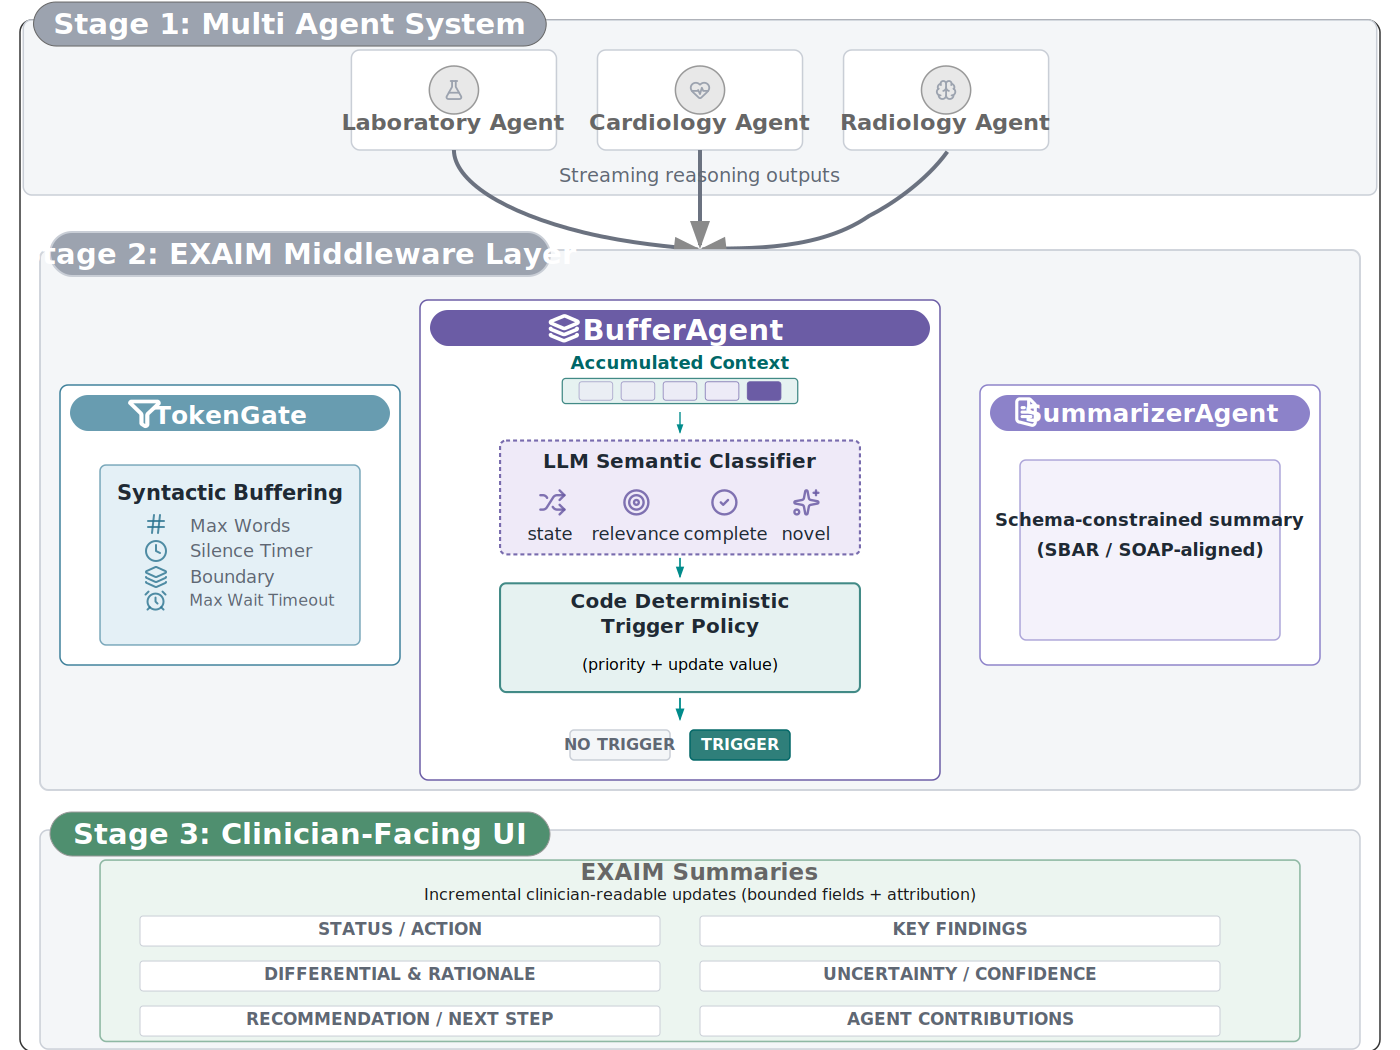
\includegraphics[width=\textwidth]{../raw/systemFigure/system.pdf}
    \caption{EXAIM middleware: converts interleaved multi-agent reasoning into concise, schema-aligned SBAR (Situation, Background, Assessment, Recommendation) and SOAP (Subjective, Objective, Assessment, Plan) summaries.}
    \label{fig:system-architecture}
\end{figure*}


\subsection{TokenGate: Syntax-Aware Stream Regulation}

The raw stream $D = \{(a_t, \tau_t)\}$ provides no linguistic boundaries: $\tau_t$ may be a single character, a word fragment, or a complete paragraph. Semantic analysis requires coherent units---complete clauses or sentences---necessitating stateful accumulation.

To maintain low latency and avoid dependencies on model-specific tokenizers (e.g., BPE, tiktoken), TokenGate operates on whitespace-delimited word counts rather than subword tokens. This design choice trades fine-grained precision for computational simplicity and cross-model portability.

TokenGate implements a stateful accumulation buffer that flushes under one of four compactly specified conditions to balance linguistic coherence and responsiveness: (1) a boundary-aware flush when the buffer has at least $w_{\text{min}}$ words and ends with terminal punctuation; (2) a hard-limit flush when the buffer exceeds $w_{\text{max}}$ words regardless of punctuation; (3) a silence timeout flush if the agent is silent for more than $t_{\text{silence}}$ seconds while the buffer contains at least $w_{\text{min}}$ words; and (4) a max wait timeout flush if total wait time surpasses $t_{\text{max}}$ since the first delta. These parameters (min\_words, max\_words, t\_silence, t\_max) jointly determine the Pareto frontier between linguistic coherence and real-time responsiveness. Section~\ref{sec:calibration} describes the systematic calibration procedure used to identify optimal values.

\subsection{BufferAgent: Semantic Event Detection}

If TokenGate solves the syntactic segmentation problem, BufferAgent solves the semantic filtering problem. Not every coherent chunk warrants triggering a summary: content may restate prior conclusions or explore already-addressed hypotheses. Unfiltered presentation would violate the first design objective (minimize update frequency).

The BufferAgent implements semantic buffering. It evaluates incoming token chunks against a sliding window of recent summaries to predict four boolean states

\begin{enumerate}
\item $\mathit{complete}$: Chunk exhibits phrase-level structural closure (finished clause, action statement, or sentence boundary)
\item $\mathit{relevant}$: Content contributes interruption-worthy clinical value (diagnostic shifts, abnormal findings, or action changes)
\item $\mathit{novel}$: Content introduces substantive information not already captured in recent summaries
\item $\mathit{state} \in \{\text{SAME\_TOPIC\_CONTINUING}, \text{SHIFT}, \text{CRITICAL}\}$: Topic continuity classification
\end{enumerate}

These feed a deterministic trigger decision:
\begin{equation}
T = \begin{cases}
\text{True} & \text{if } \mathit{State} = \text{CRITICAL} \\
\text{True} & \text{if } \mathit{Complete} \land \mathit{Relevant} \land \mathit{Novel} \\
\text{True} & \text{if } (\mathit{State} = \text{SHIFT}) \land \mathit{Relevant} \land \mathit{Novel} \\
\text{False} & \text{otherwise}
\end{cases}
\end{equation}

This encodes a hypothesis that clinicians need immediate critical alerts and topic transitions---but not incremental deliberation. Crucially, the \textit{State} = \text{CRITICAL} condition serves as a safety fail-safe, bypassing the novelty filter to ensure that potential safety threats are never suppressed by redundancy checks. Novelty is otherwise assessed against prior summaries rather than raw trace content, which prevents redundant updates at the output level and stabilizes clinician-facing update behavior.

When $T = \text{False}$, the chunk is retained in BufferAgent's internal accumulator rather than discarded. Subsequent chunks are appended to this buffer, and when a future chunk satisfies the trigger condition, all accumulated segments are flushed together to SummarizerAgent. This ensures that suppressed content is not lost but consolidated into the next triggered update, preserving information continuity while maintaining sparse interruption patterns.

This hybrid Neuro-Symbolic approach ensures that stochastic LLM reasoning is bounded by deterministic workflow rules.

\subsection{SummarizerAgent: Schema-Constrained Synthesis}

When BufferAgent determines that a chunk merits clinician attention, SummarizerAgent faces the final transformation challenge: compressing potentially verbose agent reasoning into a rigid, scannable format aligned with clinical communication standards. This component embodies the system's commitment to interface stability---no matter how chaotic or verbose the upstream reasoning, the output must conform to a bounded schema that downstream UIs can reliably render.

The agent receives three inputs: the triggering chunk $C$, the agent context (identifier and role), and a sliding window of the three most recent summaries $H_{k=3}$. This limited history serves dual purposes---it enables the summarizer to avoid repeating recently stated information while providing continuity for multi-turn reasoning threads.

Generation employs a three-attempt validation strategy to guarantee schema compliance. The LLM first generates structured output using strict Pydantic type definitions with schema enforcement (strict=True) mapped to SBAR/SOAP fields (Table~\ref{tab:schema}). If character limits are exceeded, the system creates a targeted rewrite prompt identifying the violating fields and their required length reductions, then re-invokes the LLM. Should validation still fail after this rewrite attempt, the system applies a conservative fallback truncation to enforce schema limits; importantly, EXAIM records raw token-level traces (and exposes trace callbacks) so the pre-truncation content is preserved for post-hoc inspection and auditing.

This schema-first approach differs fundamentally from unconstrained summarization, which optimizes for semantic coverage or fluency but provides no length guarantees. EXAIM inverts this priority: the AgentSummary schema (Table~\ref{tab:schema}) enforces a structured contract between the middleware and clinician-facing interfaces, mapping each field to configurable clinical communication frameworks (e.g., SBAR/SOAP). While we evaluate a fixed schema here, the artifact supports injecting site-specific JSON definitions to align with local EHR documentation standards. Character budgets are non-negotiable constraints derived from UI layout requirements---brief field lengths force scannability, field semantics mirror clinical documentation workflows, and hard limits guarantee stable UI footprint regardless of model verbosity.

\begin{table*}[htbp]
\caption{EXAIM Summary Schema: Clinical Mapping and Bounded Output Budgets}
\label{tab:schema}
\begin{center}
\renewcommand{\arraystretch}{1.3}
\begin{tabular}{p{2.5cm}p{2.5cm}p{4cm}p{1.5cm}p{4.5cm}}
\toprule
\textbf{Field} & \textbf{Clinical Map} & \textbf{Role} & \textbf{Budget (Chars)} & \textbf{Design Motivation} \\
\midrule
Status / Action & SBAR: Situation & Alert header; scannable update. & 150 chars & Enforces scannability via brief title heuristic \cite{pourian2025alerts}. \\
Key Findings & SOAP: Obj/Subj & Salient facts; ``live snippet'' paradigm. & 180 chars & Supports $\sim$2 concise snippets aligned with targeted summarization limits \cite{vanveen2023summarization}. Structured presentation addresses transparency barriers identified in patient-centered CDSS deployment \cite{harrison2022patient}. \\
Differential & SOAP: Assessment & Diagnostic interpretation. & 210 chars & Bounds complexity to maintain interpretability \cite{lage2019interpretability}. \\
Uncertainty & SOAP: Assessment & Explicit confidence signal. & 120 chars & Simplified framing for trust calibration \cite{goel2022covid}. \\
Rec. / Plan & SOAP: Plan & Actionable next step. & 180 chars & Action-linked explanations \cite{silva2023xai}. \\
Agent Contrib. & System Meta & Attribution of active agents. & 150 chars & Pipeline transparency patterns \cite{donadello2021sexai}. \\
\bottomrule
\end{tabular}
\end{center}
\end{table*}

\subsection{Demonstrative Case Walkthrough}

We illustrate the system's noise-reduction capability using a specific interaction sequence from Case ID 33651373 (trace generated as described in Section~\ref{sec:data}; Fig.~\ref{fig:suppression-demo}). Prior to this snapshot, doctor0 and doctor1 had established Spinocerebellar Ataxia (SCA) as the leading diagnosis. doctor2 subsequently entered the discussion with a verbose concurrence (visible in Fig.~\ref{fig:suppression-demo}) which, while clinically accurate, merely restated the consensus.

As visualized in the BufferAgent status card (Fig.~\ref{fig:logic-card}), the middleware decomposed this stream into semantic flags. Although the content was classified as Relevant and Complete, the novelty filter flagged it as Novel=False because the diagnostic conclusion matched the active summary state. Consequently, EXAIM suppressed the interruption, keeping the clinician-facing dashboard stable. The system continued to buffer silently until doctor2 introduced specific new evidence regarding ``High-Resolution MRI techniques'' and ``Oligoclonal bands,'' which finally triggered a consolidated, high-density update.

\begin{figure}[h]
    \centering
    \scalebox{0.65}{%
    \begin{tcolorbox}[
        enhanced,
        colback=white,
        colframe=black,
        boxrule=0.5mm,
        arc=2mm,
        drop shadow,
        left=4mm,
        right=4mm,
        top=2mm,
        bottom=2mm,
        title=\textbf{BufferAgent Status [doctor2]},
        fonttitle=\bfseries\normalsize,
        coltitle=black,
        colbacktitle=white,
        halign title=center,
        fontupper=\normalsize
    ]
        \normalsize
        
        \textbf{Input Stream:}
        \vspace{-1mm}
        \begin{quote}
            \itshape "...I concur with both doctor0 and doctor1... adding no new information."
        \end{quote}
        \vspace{1.5mm}
        
        \textbf{Decision Flags:}
        \vspace{0.5mm}
        
        \begin{center}
        \begin{tabular}{@{}c@{}}
            \raisebox{5pt}{State} \\
            \tcbox[colback=churkinpurple!15, colframe=churkinpurple, size=small, boxrule=0.5mm, left=2mm, right=2mm, top=0.5mm, bottom=0.5mm, fontupper=\normalsize]{\textcolor{churkinpurple}{\texttt{SAME\_TOPIC\_CONTINUING}}}
        \end{tabular}
        \end{center}
        
        \vspace{0.1mm}
        \begin{center}
        \begin{tabular}{@{}c@{\hspace{2mm}}c@{\hspace{2mm}}c@{}}
            \begin{tabular}{@{}c@{}}
                \raisebox{5pt}{Complete} \\[-3pt]
                \tcbox[colback=statusgreen!15, colframe=statusgreen, size=small, boxrule=0.5mm, left=2mm, right=2mm, top=0.2mm, bottom=0.2mm, fontupper=\normalsize]{\textcolor{statusgreen}{\textbf{True}}}
            \end{tabular} &
            \begin{tabular}{@{}c@{}}
                \raisebox{5pt}{Relevant} \\[-3pt]
                \tcbox[colback=statusgreen!15, colframe=statusgreen, size=small, boxrule=0.5mm, left=2mm, right=2mm, top=0.2mm, bottom=0.2mm, fontupper=\normalsize]{\textcolor{statusgreen}{\textbf{True}}}
            \end{tabular} &
            \begin{tabular}{@{}c@{}}
                \raisebox{5pt}{Novel} \\[-3pt]
                \tcbox[colback=statusred!15, colframe=statusred, size=small, boxrule=0.5mm, left=2mm, right=2mm, top=0.2mm, bottom=0.2mm, fontupper=\normalsize]{\textcolor{statusred}{\textbf{False}}}
            \end{tabular} \\
        \end{tabular}
        \end{center}
        \vspace{-2mm}
        \begin{center}
            $\downarrow$
        \end{center}
        \vspace{-2mm}
        \begin{center}
            \tcbox[
                enhanced,
                colback=statusred!20,
                colframe=statusred,
                boxrule=0.5mm,
                size=normal,
                fontupper=\bfseries\normalsize,
                left=3mm,
                right=3mm,
                top=0.5mm,
                bottom=0.5mm
            ]{\textcolor{statusred}{Trigger = False (Suppressed)}}
        \end{center}
        
        \vspace{0.1mm}
        \noindent\rule{\linewidth}{0.5mm}
        \vspace{0.5mm}
        
        \textbf{Rationale:} doctor2 concurs with SCA based on ataxia/dysarthria/MRI... adding no new information. The content is \textcolor{statusgreen}{relevant} as it details planned actions, but it is \textcolor{statusred}{not novel} as these details were already broadly mentioned in previous summaries.
    \end{tcolorbox}%
    }
    \caption{BufferAgent System Status Card showing the hierarchical decision logic.}
    \label{fig:logic-card}
\end{figure}

\begin{figure*}[htbp]
\centering
\scalebox{1}{%
\includegraphics[width=\textwidth]{case_walkthrough/CaseWalkthroughImage.png}%
}
\caption{EXAIM dashboard during redundancy suppression: the incoming raw stream (left) is suppressed, leaving the displayed summary (right) unchanged.}
\label{fig:suppression-demo}
\end{figure*}

\section{Experiments and Results}
\label{sec:experiments}

We verify the effectiveness of the EXAIM artifact through a controlled ablation study using deterministic replays of multi-agent reasoning traces. This deterministic replay protocol ensures identical input conditions across ablations, allowing us to rigorously quantify the trade-off between update frequency and semantic coverage. Consequently, this evaluation functions as an architectural stress test, utilizing rare-disease diagnostic traces---which generate significantly higher reasoning volume and interleaved noise than routine cases---to establish the system's performance boundaries under extreme operational conditions.
\subsection{Data / Trace Replay Setup}
\label{sec:data}

We utilized the Multi-Agent Conversation (MAC) framework \cite{chenx2025diagnostic} as the upstream trace generator. MAC is a multi-agent diagnostic system where diverse doctor agents and a supervisor collaborate to solve complex medical cases. We executed MAC with GPT-4o-mini using the authors' default configuration without modification.

To capture realistic streaming dynamics, we instrumented MAC via a transparent OpenAI API monkeypatch that logs per-delta emissions and microsecond timestamps without altering MAC's conversation logic, speaker selection, or termination behavior. These logs serve as a frozen replay dataset of 40 rare-disease diagnostic cases from MAC's dataset (seed=42), enabling deterministic simulation of live streams.

EXAIM uses Google Gemini (gemini-2.5-flash-lite) for both BufferAgent semantic classification and SummarizerAgent schema-constrained generation. Middleware inference was executed deterministically (temperature=0.0), with other parameters left at defaults. Prompts and decoding parameters are fixed and available in the repository.

Unified Medical Language System (UMLS) concepts (CUIs) used for metric computation were extracted with scispaCy (model = en\_core\_sci\_sm) linked to UMLS Release 2023AB; extraction applied a candidate-score threshold ($\geq 0.7$), top-K selection (K=10), and stoplist filtering for entities and CUIs.

We report all text volume and budget-normalized metrics using Character-Normalized Token Units (CTU), defined as $\lceil\text{len(text)}/4\rceil$, a deterministic and vendor-agnostic normalization unit applied uniformly to both trace inputs and summary outputs to enable fair and reproducible cross-variant comparison.

\subsection{Ablation and Baselines}
\label{sec:ablation}

We isolate the contribution of each architectural primitive through a controlled ablation study. V1 establishes a turn-boundary baseline, summarizing only when agents complete their generations---a natural structural trigger reflecting conventional dialogue system paradigms. V2 disables BufferAgent filtering entirely, passing all TokenGate flushes directly to summarization to isolate the impact of semantic gating on update frequency and redundancy. V3 replaces TokenGate's syntax-aware segmentation with calibrated fixed-interval chunking, testing whether adaptive linguistic boundaries improve entity grounding over uniform partitioning. V4 disables only the novelty filter while preserving BufferAgent's completeness and relevance checks, isolating whether contextual redundancy detection is necessary for managing update frequency. Table~\ref{tab:ablation-variants} defines the five experimental configurations (V0--V4).

\begin{table}[htbp]
\caption{Ablation Variant Configurations}
\label{tab:ablation-variants}
\begin{center}
\renewcommand{\arraystretch}{1.3}
\begin{tabular}{lcccc}
\toprule
\textbf{Variant} & \textbf{TokenGate} & \textbf{BufferAgent} & \textbf{Novelty} \\
\midrule
V0 (Full EXAIM) & \checkmark & \checkmark & \checkmark\\
V1 (Turn-End) & $\times$ & $\times$ & N/A \\
V2 (No BufferAgent) & \checkmark & $\times$ & N/A \\
V3 (Fixed-Chunk) & $\times$ & \checkmark & \checkmark \\
& (fixed CTU) & & & \\
V4 (No Novelty) & \checkmark & \checkmark & $\times$ \\
\bottomrule
\end{tabular}
\end{center}
\footnotesize
Note: All variants use identical SummarizerAgent schema and history\_k=3 for fair comparison.
\normalsize
\end{table}

\subsection{Calibration Protocol}
\label{sec:calibration}
 
To ensure fair evaluation, we executed a rigorous parameter selection process before final testing. First, we calibrated the TokenGate module by performing a grid search over 625 policy combinations (varying word counts and timeouts) on the replay dataset. The final policy (min\_words=60, max\_words=100, t\_silence=1.0~s, t\_max=4.0~s) was selected via Pareto frontier analysis to jointly optimize latency and linguistic coherence. Second, we established the V3 Fixed-Chunk parameters by deriving the chunk size from V0 TokenGate regular flushes (excluding end-of-trace and turn-end) using a two-stage median: calculating the per-case median CTU, followed by the median across the first 40 cases. This ensures V3 operates at comparable segmentation granularity to V0 while isolating the contribution of adaptive boundaries.


\subsection{Metrics}

We prioritized seven metrics (M3, M4, M5, M6, M7, M8, M10) that directly quantify utility and reliability proxies:

\begin{itemize}
    \item \textbf{Entity Grounding (M6) (referred to as ``faithfulness'' in the released artifact):} The fraction of summary concepts grounded in the full trace:
    \begin{equation}
    M6 = \frac{|\text{summary\_CUIs} \cap \text{trace\_CUIs}|}{|\text{summary\_CUIs}|}.
    \end{equation}
    Higher scores indicate stronger concept-level grounding.

    \item \textbf{Window-Groundedness (M7):} A window-grounded variant of entity grounding that measures the fraction of summary concepts grounded within a local sliding window of trace content centered on the summary's trigger:
    \begin{equation}
    M7 = \frac{1}{N}\sum_{i=1}^{N} \frac{|\text{summary\_CUIs}_i \cap \text{trace\_CUIs}_{\text{window}(i)}|}{|\text{summary\_CUIs}_i|},
    \end{equation}
    where $N$ is the number of evaluated summaries, $\text{summary\_CUIs}_i$ is the set of CUIs extracted from summary $i$, and $\text{trace\_CUIs}_{\text{window}(i)}$ denotes the set of CUIs extracted from the sliding window of trace content surrounding the trigger that produced summary $i$. M7 reflects local grounding and is less sensitive to distant context than M6.
    \item \textbf{Redundancy Reduction (M3):} Measured via mean Jaccard similarity between consecutive summary updates:
    \begin{equation}
    M3 = \frac{1}{n-1}\sum_{i=1}^{n-1} \frac{|C_i \cap C_{i+1}|}{|C_i \cup C_{i+1}|},
    \end{equation}
    where $C_i$ and $C_{i+1}$ are the sets of unique UMLS concepts (CUIs) extracted from summaries $S_i$ and $S_{i+1}$, and $n$ is the total number of summaries. Lower scores indicate successful suppression of repetitive content.
    \item \textbf{Trace Coverage (M4):} The fraction of unique trace CUIs captured across all summaries:
    \begin{equation}
    M4 = \frac{|\bigcup_{i=1}^{n} \text{summary\_CUIs}_i \cap \text{trace\_CUIs}|}{|\text{trace\_CUIs}|}.
    \end{equation}
    This metric measures aggregate coverage across all summaries.

    \item \textbf{Budget-Constrained Coverage (M5):} Coverage attainable within a fixed reader budget $B$ (measured in Character-Normalized Token Units, CTU).
    \begin{equation}
    k(B)=\max\left\{m:\sum_{i=1}^{m}\text{ctu}_i \le B\right\}.
    \end{equation}
    
    Then
    \begin{equation}
    \text{M5}(B)=\frac{\left|\bigcup_{i=1}^{k(B)}\text{summary\_CUIs}_i \cap \text{trace\_CUIs}\right|}{\left|\text{trace\_CUIs}\right|},
    \end{equation}
    where $\text{ctu}_i$ denotes the Character\-Normalized Token Units of summary $i$, $B$ is the total output budget in CTU, summaries are ordered by emission time, and $k(B)$ is the largest prefix of summaries whose cumulative CTU does not exceed $B$.
    
    \item \textbf{System Latency (M8):} The end-to-end processing time (buffer analysis + summarization generation).
    \item \textbf{Schema Compliance (M10):} The rate of successful adherence to the JSON clinical output schema.
\end{itemize}
Note on concept-based metrics: Because M3--M7 rely on explicit entity extraction, they may under-score schema-constrained summaries when clinically valid content is expressed via abbreviations, paraphrases, or normalization (e.g., ``acute renal failure'' $\rightarrow$ ``AKI''), a limitation typical of extraction/matching-based concept metrics \cite{vanveen2023summarization}; however, they remain appropriate for relative comparison across ablation variants under identical extraction assumptions.

Supplementary metrics (M1: Update Count; M2: Output Volume (CTU); M9: LLM Usage (CTU)) provide context for trade-off analysis.

\subsection{Results}

We report four key findings from the controlled ablation across 40 MAC replay cases. All confidence intervals are 95\% bootstrap (10,000 samples, seed=42).

\textbf{Finding 1 (RQ1a, RQ1b): Semantic buffering reduces interruption frequency by 75\% while preserving competitive coverage at clinician-realistic budgets.} V0 (full EXAIM) generates 11.65 updates per case vs. V2 (no BufferAgent) with 46.4 updates (paired $\Delta = -34.75$ [CI: -35.1, -34.4]). Despite raw coverage disadvantage (M4: V0 = 0.162 vs. V2 = 0.312), V0 achieves 0.129 coverage at $\le 1000$ CTU budget vs. V2's 0.134 (Fig.~\ref{fig:budget-coverage}), demonstrating that semantic gating trades volume for efficiency without compromising information yield at realistic reading limits.

Information density further illustrates V0's efficiency: V0 achieves Coverage/Update = 0.0139 vs. V2 = 0.0067 (paired $\Delta = +0.0072$ [CI: +0.0065, +0.0079]), indicating V0 delivers roughly 2$\times$ semantic yield per clinician-facing interruption. V2's 4$\times$ update burden (46.4 vs. 11.65) without proportional coverage gain illustrates the high volume of the "firehose" baseline.

\textbf{Finding 2 (RQ1c, RQ1d): Syntax-aware buffering improves entity grounding compared to structural triggers.} V0 achieves M6 (strict entity grounding) = 0.421 [0.389, 0.453] vs. V1 (turn-end) = 0.333 [0.309, 0.356], a 26\% improvement. This suggests TokenGate's linguistic segmentation produces more groundable content for summarization than turn-boundary triggers. Window-groundedness (M7) remains high across variants (V0 = 0.825), indicating summaries stay locally grounded within trigger windows despite NER under-scoring schema-constrained paraphrases.

\textbf{Finding 3 (RQ1b): Novelty filtering is necessary to manage interruption burden.} V4 (no novelty) generates 16.45 updates vs. V0's 11.65 (41\% increase), with marginal coverage gain (M4: V4 = 0.175 vs. V0 = 0.162, 8\% relative). Redundancy metrics (M3) confirm V0 (0.366) and V4 (0.346) achieve similar consecutive-summary overlap, but V0's lower update count indicates novelty filtering suppresses low-information triggers without harming redundancy control.

\textbf{Finding 4 (RQ1c): Schema compliance and latency support real-time feasibility.} Schema compliance (M10) exceeds 95\% across all variants (V0 = 0.968), validating strict Pydantic-like validation. Median latency for V0 is 1.22~s (P95 = 1.84~s), confirming asynchronous sidecar architecture preserves real-time responsiveness. Latency decomposition shows V0's added processing time (~0.2~s over V1) arises from BufferAgent semantic classification, reflecting an explicit compute-for-interruption-reduction trade-off.

 
\begin{table*}[t]
\centering
\caption{Contract and Quality Metrics (Mean [95\% CI])}
\label{tab:metrics}
\renewcommand{\arraystretch}{1.25} % Adds vertical space between rows
\setlength{\tabcolsep}{6pt}        % Adds horizontal space between columns

\begin{tabular}{l c c c c c}
\toprule  % Professional top line
\textbf{Metric} & \textbf{V0} & \textbf{V1} & \textbf{V2} & \textbf{V3} & \textbf{V4} \\
\midrule  % Professional middle line

Entity Grounding \textit{(M6)} & 0.421 & 0.333 & 0.409 & 0.382 & 0.424 \\
& [0.389, 0.453] & [0.309, 0.356] & [0.382, 0.437] & [0.353, 0.413] & [0.395, 0.454] \\
\addlinespace[8pt]

Window-Groundedness \textit{(M7)} & 0.825 & 0.787 & 0.879 & 0.823 & 0.845 \\
& [0.807, 0.842] & [0.763, 0.810] & [0.869, 0.890] & [0.799, 0.846] & [0.829, 0.862] \\
\addlinespace[8pt]

Trace Coverage \textit{(M4)} & 0.162 & 0.144 & 0.312 & 0.134 & 0.175 \\
& [0.148, 0.175] & [0.135, 0.153] & [0.296, 0.328] & [0.120, 0.149] & [0.158, 0.192] \\
\midrule

% Single value rows don't need the split
Redundancy Reduction \textit{(M3)} & 0.366 & 0.456 & 0.348 & 0.413 & 0.346 \\
Schema Compliance \textit{(M10)} & 0.968 & 0.968 & 0.975 & 0.958 & 0.950 \\
\midrule

Latency \textit{(M8, seconds)} & & & & & \\
\hspace{3mm} Mean & 1.28 & 1.03 & 1.14 & 1.07 & 1.37 \\
\hspace{3mm} Median & 1.22 & 0.96 & 1.06 & 1.04 & 1.33 \\
\hspace{3mm} P95 & 1.84 & 1.59 & 1.91 & 1.52 & 2.12 \\
\bottomrule % Professional bottom line
\end{tabular}
\end{table*}
 
Tables~\ref{tab:metrics} and~\ref{tab:operational-density} provide complete metric breakdowns. Table~\ref{tab:paired-bootstrap} reports statistical comparisons.

\begin{table}[htbp]
\caption{Operational Burden, Resource Consumption, and Information Density}
\begin{center}
\resizebox{\columnwidth}{!}{%
\renewcommand{\arraystretch}{1.3}
\begin{tabular}{lccccc}
\toprule
\textbf{Metric} & \textbf{V0} & \textbf{V1} & \textbf{V2} & \textbf{V3} & \textbf{V4} \\
\midrule
Update Count (M1) & 11.65 & 8.5 & 46.4 & 9.5 & 16.45 \\
Output Volume (M2, CTU) & 1391 & 1148 & 4313 & 1156 & 1763 \\
LLM Usage (M9, CTU) & 62178 & 11618 & 37151 & 81694 & 58605 \\
\midrule
Coverage/Update & 0.0139 & 0.0169 & 0.0067 & 0.0141 & 0.0107 \\
\bottomrule
\end{tabular}
}
\label{tab:operational-density}
\end{center}
\footnotesize
\normalsize
\end{table}


To evaluate information density---the core utility trade-off between coverage and burden---we compute efficiency metrics normalized by update count and output volume (Table~\ref{tab:operational-density}). Additionally, Fig.~\ref{fig:budget-coverage} shows M5 coverage across multiple CTU budgets, revealing V0's competitive performance at clinician-realistic reading budgets ($\leq$1000 CTU).

% Information density rows merged into Table~\ref{tab:operational-density}.

\begin{figure}[htbp]
\centering
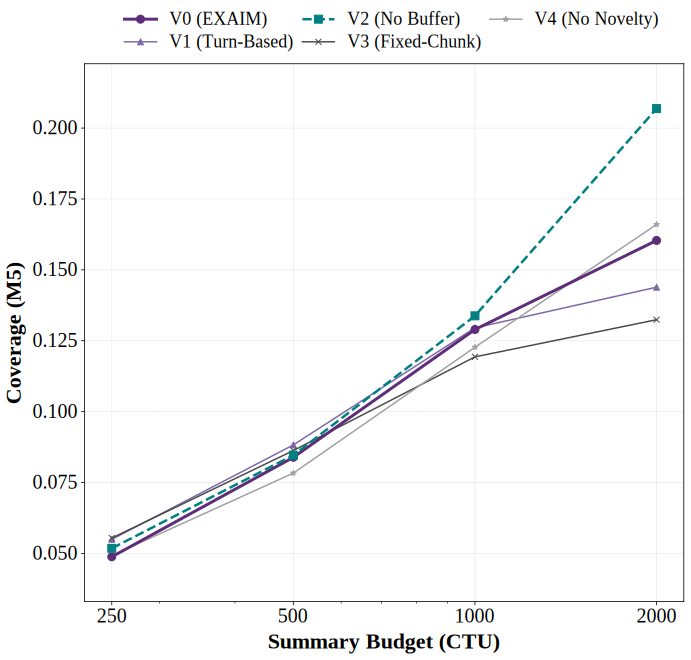
\includegraphics[width=\columnwidth]{saturation/saturation.pdf}
\caption{Budget-Constrained Coverage (M5). V0 (EXAIM) saturates early; V2 diverges at high budgets.}
\label{fig:budget-coverage}
\end{figure}


To support headline claims with rigorous statistical evidence, we computed paired differences (V0 minus comparator) across the 40 replay cases, bootstrapping to estimate 95\% confidence intervals (Table~\ref{tab:paired-bootstrap}).

\begin{table}[htbp]
\caption{Paired Bootstrap Comparisons}
\begin{center}
\resizebox{\columnwidth}{!}{%
\renewcommand{\arraystretch}{1.3}
\begin{tabular}{lcc}
\toprule
\textbf{Comparison} & \textbf{$\Delta$ Update Count (M1)} & \textbf{$\Delta$ Coverage/Update} \\
\midrule
V0 -- V2 (mean) & --34.75 & +0.0072 \\
CI [low, high] & [--35.1, --34.4] & [+0.0065, +0.0079] \\
\midrule
V0 -- V1 (mean) & +3.15 & --0.0030 \\
CI [low, high] & [+2.9, +3.4] & [--0.0038, --0.0022] \\
\bottomrule
\end{tabular}
}
\label{tab:paired-bootstrap}
\end{center}
\footnotesize
Note: Paired bootstrap: 10,000 samples, seed=42.
\normalsize
\end{table}



\section{Discussion}

\subsection{Theoretical Implications: Extremes as Design Anchors}

This study extends Design Science Research (DSR) in clinical AI by formalizing the "transparency paradox" as a manageable control problem. 
Historically, CDSS design has oscillated between two extremes: opaque black boxes (high efficiency, low trust) and "firehose" transparency (high trust, cognitive failure). Our ablation results (V0 vs V1/V2) introduce a third stable state: \textbf{Semantic State Transparency}.
By shifting the unit of explanation from the \textit{architectural turn} to the \textit{clinical semantic event}, EXAIM demonstrates that transparency is not a fixed attribute of the model but a tunable variable of the interface. This provides a theoretical design anchor for future multi-agent interfaces: explainability should be decoupled from generation mechanics and governed by an independent logic of clinical meaningfulness.

\subsection{Practical Implications for Workflow Integration}

The V4 ablation exposes a fundamental mismatch between generative AI architectures and clinical information needs. In the absence of novelty filtering, V4 produces 41\% more updates with negligible coverage gains, revealing that LLM token generation operates under a ``Shannon entropy'' regime---maximizing statistical variation---while clinical decision-making requires ``semantic value'' selection---identifying state-changing information. This distinction has direct architectural implications: CDSS interfaces must transition from \textit{generative} paradigms (where more output is presumed better) to \textit{synthesizing} paradigms (where middleware actively suppresses redundancy). 

Operationally, our results suggest that deploying multi-agent CDSS without intermediate semantic filtering could impose excessive information burden on time-constrained clinicians. The observed update reduction offloads the task of filtering from clinicians to automated middleware, directly addressing workflow compatibility barriers identified in recent CDSS reviews \cite{bayor2025cdss}. Critically, ``novelty'' is not a static property of text but a contextual relationship between incoming content and recent clinical state---a design principle that should inform all streaming AI transparency layers.

\subsection{Deployment Considerations}

To move from artifact to operation, we instantiate EXAIM using a four-tier architecture adapted from recent generative AI patterns. This structure ensures robustness by decoupling the probabilistic reasoning of the agents from the deterministic requirements of the EHR interface:
\begin{enumerate}
    \item \textbf{Data Layer}: Integration with FHIR-enabled EHRs to feed live patient context to upstream agents.
    \item \textbf{Model Layer}: Hosting the multi-agent reasoning engine (e.g., MAC) in a secure, HIPAA-compliant enclave.
    	\item \textbf{Middleware Layer}: Deploying EXAIM as a low-latency interaction gateway. This layer handles the "contract" capability ensuring predictable JSON output. From a governance perspective, EXAIM functions as a "View Layer"; the raw agent trace (Stage 1) must be persisted independently as the immutable legal record for auditability.
    \item \textbf{User Layer}: A React/Web-based clinician dashboard that subscribes to the EXAIM JSON stream, rendering cards that update in place.
\end{enumerate}
\subsection{Limitations and Boundary Conditions}

This study prioritizes architectural control over ecological validity by evaluating EXAIM on frozen, deterministic trace replays (40 MAC cases), which isolates middleware flow-control effects from human interaction dynamics. Generalization is currently limited to the MAC/GPT-4o-mini upstream topology; performance under other agent frameworks or model families remains untested. As a result, we do not measure longitudinal workflow phenomena (e.g., alert-fatigue adaptation, trust trajectories), and any burden-related benefits are proxy inferences from interruption and budgeted-coverage metrics rather than observed clinical outcomes. A second limitation is a safety risk introduced by the LLM-based semantic gating: misclassification can hide clinically meaningful disagreement between agents (e.g., conflict mislabeled as redundancy).  We do not quantify suppression errors or implement boundary-aware fail-safes in the current artifact.
\section{Conclusion and Future Work}

This work presented EXAIM, a middleware architecture that resolves the lack of semantic event-driven buffering in multi-agent diagnostic traces by introducing a three-stage pipeline: TokenGate (syntax-aware stream regulation), BufferAgent (semantic event detection), and SummarizerAgent (schema-constrained synthesis).

As healthcare transitions toward "Agentic" workflows, the volume of machine-generated reasoning is outpacing human cognitive capacity. To our knowledge, EXAIM represents the first middleware solution designed specifically for the live summarization of interleaved multi-agent traces. While prior systems have successfully addressed summarization of dyadic doctor-patient dialogue \cite{leduc2025speech,zhang2024annotate,krishna2021soap}, these approaches rely on structural triggers that falter in the high-velocity, asynchronous context of collaborative multi-agent reasoning.

By introducing Semantic State Transparency, this work challenges the prevailing design assumption that transparency requires exposing the raw token stream. Instead, we demonstrate that effective human-AI collaboration requires decoupling the agent's generation rate from the clinician's consumption capacity. The middleware's ability to filter reasoning based on semantic novelty rather than arbitrary time windows establishes a new architectural primitive for CDSS: the "semantic governor."

Future work will advance the artifact along three maturity axes. First, we will move from offline replay to shadow-mode evaluation alongside live workflows to measure workflow endpoints (e.g., time-to-decision) without influencing clinician decisions. Second, we will harden safety against inherent problems imposed by the LLM-based semantic gating by adding trace-grounding verification and implementing a "shadow mode" deployment to quantify False Negative suppression rates against human adjudication, ensuring critical inter-agent disagreements are never silently filtered. Third, establishing regulatory compliance by generating structured audit trails that document summary provenance, grounding verification status, and unresolved conflicts, meeting transparency and accountability requirements to support deployment-grade accountability. Collectively, these extensions will transform EXAIM from a validated proof-of-concept into a deployable clinical artifact that manages the transparency-efficiency trade-off under human cognitive constraints.

\section*{Acknowledgment}


The authors thank the MAC framework developers for making their diagnostic reasoning traces available for instrumentation.

\section*{Artifact Availability}
The complete EXAIM research artifact which includes source code, configuration files, evaluation scripts, and trace-replay infrastructure used in this study is publicly archived on Zenodo~\cite{abem_woldesenbet_2026_18319043}.

\bibliographystyle{IEEEtran}
\bibliography{references}

\end{document}





